\documentclass{standalone}
\usepackage{tikz}
\usetikzlibrary{patterns, positioning}

\begin{document}
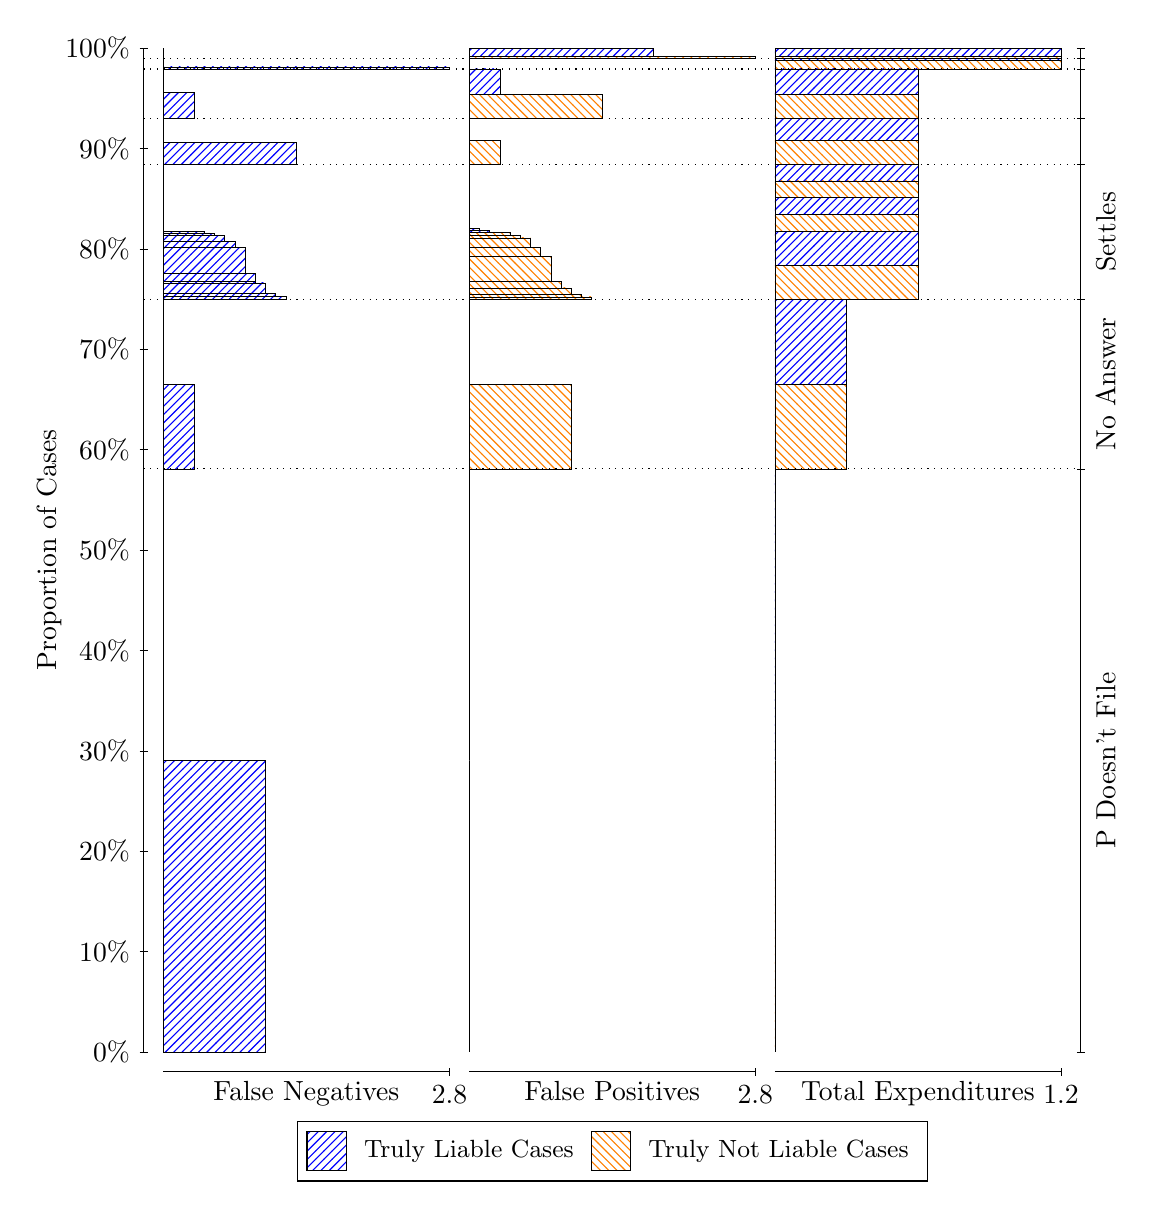
\begin{tikzpicture}
\draw[black, very thin] (1.5,1.75) -- (1.5,14.5);
\node[rotate=90, anchor=center] at (0.3, 8.125) {Proportion of Cases};
\draw[black, very thin] (1.45,1.75) -- (1.55,1.75);
\node[anchor=east] at (1.45, 1.75) {0\%};
\draw[black, very thin] (1.45,3.025) -- (1.55,3.025);
\node[anchor=east] at (1.45, 3.025) {10\%};
\draw[black, very thin] (1.45,4.3) -- (1.55,4.3);
\node[anchor=east] at (1.45, 4.3) {20\%};
\draw[black, very thin] (1.45,5.575) -- (1.55,5.575);
\node[anchor=east] at (1.45, 5.575) {30\%};
\draw[black, very thin] (1.45,6.85) -- (1.55,6.85);
\node[anchor=east] at (1.45, 6.85) {40\%};
\draw[black, very thin] (1.45,8.125) -- (1.55,8.125);
\node[anchor=east] at (1.45, 8.125) {50\%};
\draw[black, very thin] (1.45,9.4) -- (1.55,9.4);
\node[anchor=east] at (1.45, 9.4) {60\%};
\draw[black, very thin] (1.45,10.675) -- (1.55,10.675);
\node[anchor=east] at (1.45, 10.675) {70\%};
\draw[black, very thin] (1.45,11.95) -- (1.55,11.95);
\node[anchor=east] at (1.45, 11.95) {80\%};
\draw[black, very thin] (1.45,13.225) -- (1.55,13.225);
\node[anchor=east] at (1.45, 13.225) {90\%};
\draw[black, very thin] (1.45,14.5) -- (1.55,14.5);
\node[anchor=east] at (1.45, 14.5) {100\%};

\draw[black, very thin] (13.4,1.75) -- (13.4,14.5);
\draw[black, very thin] (13.35,1.75) -- (13.45,1.75);
\node[anchor=west] at (13.35, 1.75) {};
\draw[black, very thin] (13.35,9.1553) -- (13.45,9.1553);
\node[anchor=west] at (13.35, 9.1553) {};
\draw[black, very thin] (13.35,11.311) -- (13.45,11.311);
\node[anchor=west] at (13.35, 11.311) {};
\draw[black, very thin] (13.35,13.019) -- (13.45,13.019);
\node[anchor=west] at (13.35, 13.019) {};
\draw[black, very thin] (13.35,13.61) -- (13.45,13.61);
\node[anchor=west] at (13.35, 13.61) {};
\draw[black, very thin] (13.35,14.234) -- (13.45,14.234);
\node[anchor=west] at (13.35, 14.234) {};
\draw[black, very thin] (13.35,14.372) -- (13.45,14.372);
\node[anchor=west] at (13.35, 14.372) {};
\draw[black, very thin] (13.35,14.5) -- (13.45,14.5);
\node[anchor=west] at (13.35, 14.5) {};

\draw[black, very thin, pattern color=blue, pattern=north east lines] (1.75,1.75) rectangle (3.0476,5.4526);
\draw[black, very thin, pattern color=orange, pattern=north west lines] (1.75,5.4526) rectangle (1.75,9.1553);
\draw[black, very thin, pattern color=blue, pattern=north east lines] (1.75,9.1553) rectangle (2.1393,10.233);
\draw[black, very thin, pattern color=orange, pattern=north west lines] (1.75,10.233) rectangle (1.75,11.311);
\draw[black, very thin, pattern color=blue, pattern=north east lines] (1.75,11.311) rectangle (3.3071,11.348);
\draw[black, very thin, pattern color=blue, pattern=north east lines] (1.75,11.348) rectangle (3.1774,11.381);
\draw[black, very thin, pattern color=blue, pattern=north east lines] (1.75,11.381) rectangle (3.0476,11.517);
\draw[black, very thin, pattern color=blue, pattern=north east lines] (1.75,11.517) rectangle (2.9179,11.537);
\draw[black, very thin, pattern color=blue, pattern=north east lines] (1.75,11.537) rectangle (2.9179,11.642);
\draw[black, very thin, pattern color=blue, pattern=north east lines] (1.75,11.642) rectangle (2.7881,11.965);
\draw[black, very thin, pattern color=blue, pattern=north east lines] (1.75,11.965) rectangle (2.6583,12.04);
\draw[black, very thin, pattern color=blue, pattern=north east lines] (1.75,12.04) rectangle (2.5286,12.119);
\draw[black, very thin, pattern color=blue, pattern=north east lines] (1.75,12.119) rectangle (2.3988,12.144);
\draw[black, very thin, pattern color=blue, pattern=north east lines] (1.75,12.144) rectangle (2.269,12.171);
\draw[black, very thin, pattern color=orange, pattern=north west lines] (1.75,12.171) rectangle (1.75,13.019);
\draw[black, very thin, pattern color=blue, pattern=north east lines] (1.75,13.019) rectangle (3.4369,13.3);
\draw[black, very thin, pattern color=orange, pattern=north west lines] (1.75,13.3) rectangle (1.75,13.61);
\draw[black, very thin, pattern color=blue, pattern=north east lines] (1.75,13.61) rectangle (2.1393,13.934);
\draw[black, very thin, pattern color=orange, pattern=north west lines] (1.75,13.934) rectangle (1.75,14.234);
\draw[black, very thin, pattern color=blue, pattern=north east lines] (1.75,14.234) rectangle (5.3833,14.261);
\draw[black, very thin, pattern color=orange, pattern=north west lines] (1.75,14.261) rectangle (1.75,14.372);
\draw[black, very thin, pattern color=orange, pattern=north west lines] (1.75,14.372) rectangle (1.75,14.398);
\draw[black, very thin, pattern color=blue, pattern=north east lines] (1.75,14.398) rectangle (1.75,14.5);
\draw[black, very thin, pattern color=orange, pattern=north west lines] (5.6333,1.75) rectangle (5.6333,5.4527);
\draw[black, very thin, pattern color=blue, pattern=north east lines] (5.6333,5.4527) rectangle (5.6333,9.1553);
\draw[black, very thin, pattern color=orange, pattern=north west lines] (5.6333,9.1553) rectangle (6.931,10.233);
\draw[black, very thin, pattern color=blue, pattern=north east lines] (5.6333,10.233) rectangle (5.6333,11.311);
\draw[black, very thin, pattern color=orange, pattern=north west lines] (5.6333,11.311) rectangle (7.1905,11.34);
\draw[black, very thin, pattern color=orange, pattern=north west lines] (5.6333,11.34) rectangle (7.0607,11.367);
\draw[black, very thin, pattern color=orange, pattern=north west lines] (5.6333,11.367) rectangle (6.931,11.453);
\draw[black, very thin, pattern color=orange, pattern=north west lines] (5.6333,11.453) rectangle (6.8012,11.534);
\draw[black, very thin, pattern color=orange, pattern=north west lines] (5.6333,11.534) rectangle (6.6714,11.85);
\draw[black, very thin, pattern color=orange, pattern=north west lines] (5.6333,11.85) rectangle (6.5417,11.964);
\draw[black, very thin, pattern color=orange, pattern=north west lines] (5.6333,11.964) rectangle (6.4119,12.088);
\draw[black, very thin, pattern color=orange, pattern=north west lines] (5.6333,12.088) rectangle (6.2821,12.119);
\draw[black, very thin, pattern color=orange, pattern=north west lines] (5.6333,12.119) rectangle (6.1524,12.158);
\draw[black, very thin, pattern color=blue, pattern=north east lines] (5.6333,12.158) rectangle (5.8929,12.185);
\draw[black, very thin, pattern color=blue, pattern=north east lines] (5.6333,12.185) rectangle (5.7631,12.211);
\draw[black, very thin, pattern color=blue, pattern=north east lines] (5.6333,12.211) rectangle (5.6333,13.019);
\draw[black, very thin, pattern color=orange, pattern=north west lines] (5.6333,13.019) rectangle (6.0226,13.328);
\draw[black, very thin, pattern color=blue, pattern=north east lines] (5.6333,13.328) rectangle (5.6333,13.61);
\draw[black, very thin, pattern color=orange, pattern=north west lines] (5.6333,13.61) rectangle (7.3202,13.91);
\draw[black, very thin, pattern color=blue, pattern=north east lines] (5.6333,13.91) rectangle (6.0226,14.234);
\draw[black, very thin, pattern color=orange, pattern=north west lines] (5.6333,14.234) rectangle (5.6333,14.345);
\draw[black, very thin, pattern color=blue, pattern=north east lines] (5.6333,14.345) rectangle (5.6333,14.372);
\draw[black, very thin, pattern color=orange, pattern=north west lines] (5.6333,14.372) rectangle (9.2667,14.398);
\draw[black, very thin, pattern color=blue, pattern=north east lines] (5.6333,14.398) rectangle (7.969,14.5);
\draw[black, very thin, pattern color=orange, pattern=north west lines] (9.5167,1.75) rectangle (9.5167,5.4527);
\draw[black, very thin, pattern color=blue, pattern=north east lines] (9.5167,5.4527) rectangle (9.5167,9.1553);
\draw[black, very thin, pattern color=orange, pattern=north west lines] (9.5167,9.1553) rectangle (10.425,10.233);
\draw[black, very thin, pattern color=blue, pattern=north east lines] (9.5167,10.233) rectangle (10.425,11.311);
\draw[black, very thin, pattern color=orange, pattern=north west lines] (9.5167,11.311) rectangle (11.333,11.74);
\draw[black, very thin, pattern color=blue, pattern=north east lines] (9.5167,11.74) rectangle (11.333,12.168);
\draw[black, very thin, pattern color=orange, pattern=north west lines] (9.5167,12.168) rectangle (11.333,12.383);
\draw[black, very thin, pattern color=blue, pattern=north east lines] (9.5167,12.383) rectangle (11.333,12.608);
\draw[black, very thin, pattern color=orange, pattern=north west lines] (9.5167,12.608) rectangle (11.333,12.812);
\draw[black, very thin, pattern color=blue, pattern=north east lines] (9.5167,12.812) rectangle (11.333,13.019);
\draw[black, very thin, pattern color=orange, pattern=north west lines] (9.5167,13.019) rectangle (11.333,13.328);
\draw[black, very thin, pattern color=blue, pattern=north east lines] (9.5167,13.328) rectangle (11.333,13.61);
\draw[black, very thin, pattern color=orange, pattern=north west lines] (9.5167,13.61) rectangle (11.333,13.91);
\draw[black, very thin, pattern color=blue, pattern=north east lines] (9.5167,13.91) rectangle (11.333,14.234);
\draw[black, very thin, pattern color=orange, pattern=north west lines] (9.5167,14.234) rectangle (13.15,14.345);
\draw[black, very thin, pattern color=blue, pattern=north east lines] (9.5167,14.345) rectangle (13.15,14.372);
\draw[black, very thin, pattern color=orange, pattern=north west lines] (9.5167,14.372) rectangle (13.15,14.398);
\draw[black, very thin, pattern color=blue, pattern=north east lines] (9.5167,14.398) rectangle (13.15,14.5);
\draw[black, dotted] (1.5,9.1553) -- (13.4,9.1553);
\draw[black, dotted] (1.5,11.311) -- (13.4,11.311);
\draw[black, dotted] (1.5,13.019) -- (13.4,13.019);
\draw[black, dotted] (1.5,13.61) -- (13.4,13.61);
\draw[black, dotted] (1.5,14.234) -- (13.4,14.234);
\draw[black, dotted] (1.5,14.372) -- (13.4,14.372);
\draw[black, very thin] (1.75,1.5) -- (5.3833,1.5);
\node[anchor=north] at (3.5667, 1.5) {False Negatives};
\draw[black, very thin] (5.3833,1.45) -- (5.3833,1.55);
\node[anchor=north] at (5.3833, 1.45) {2.8};

\draw[black, very thin] (5.6333,1.5) -- (9.2667,1.5);
\node[anchor=north] at (7.45, 1.5) {False Positives};
\draw[black, very thin] (9.2667,1.45) -- (9.2667,1.55);
\node[anchor=north] at (9.2667, 1.45) {2.8};

\draw[black, very thin] (9.5167,1.5) -- (13.15,1.5);
\node[anchor=north] at (11.333, 1.5) {Total Expenditures};
\draw[black, very thin] (13.15,1.45) -- (13.15,1.55);
\node[anchor=north] at (13.15, 1.45) {1.2};

\node[black, centered, rotate=90] at (13.72, 5.4527) {P Doesn't File};
\node[black, centered, rotate=90] at (13.72, 10.233) {No Answer};
\node[black, centered, rotate=90] at (13.72, 12.165) {Settles};





\draw (7.449999999999999,1.5) node[draw=none] (baseCoordinate) {};
\begin{scope}[align=center]
        \matrix[scale=0.5, draw=black, below=0.5cm of baseCoordinate, nodes={draw}, column sep=0.1cm]{
            \node[rectangle, draw, minimum width=0.5cm, minimum height=0.5cm, pattern=north east lines, pattern color=blue] {}; &
            \node[draw=none, font=\small] (B) {Truly Liable Cases}; &
            \node[rectangle, draw, minimum width=0.5cm, minimum height=0.5cm, pattern=north west lines, pattern color=orange] {}; &
            \node[draw=none, font=\small] (B) {Truly Not Liable Cases}; \\
            };
\end{scope}

\end{tikzpicture}
\end{document}